\documentclass[12pt,letterpaper]{article}
\usepackage{graphicx,textcomp}
\usepackage{natbib}
\usepackage{setspace}
\usepackage{fullpage}
\usepackage{color}
\usepackage[reqno]{amsmath}
\usepackage{amsthm}
\usepackage{fancyvrb}
\usepackage{amssymb,enumerate}
\usepackage[all]{xy}
\usepackage{endnotes}
\usepackage{lscape}
\newtheorem{com}{Comment}
\usepackage{float}
\usepackage{hyperref}
\newtheorem{lem} {Lemma}
\newtheorem{prop}{Proposition}
\newtheorem{thm}{Theorem}
\newtheorem{defn}{Definition}
\newtheorem{cor}{Corollary}
\newtheorem{obs}{Observation}
\usepackage[compact]{titlesec}
\usepackage{dcolumn}
\usepackage{tikz}
\usetikzlibrary{arrows}
\usepackage{multirow}
\usepackage{xcolor}
\newcolumntype{.}{D{.}{.}{-1}}
\newcolumntype{d}[1]{D{.}{.}{#1}}
\definecolor{light-gray}{gray}{0.65}
\usepackage{url}
\usepackage{listings}
\usepackage{color}

\definecolor{codegreen}{rgb}{0,0.6,0}
\definecolor{codegray}{rgb}{0.5,0.5,0.5}
\definecolor{codepurple}{rgb}{0.58,0,0.82}
\definecolor{backcolour}{rgb}{0.95,0.95,0.92}

\lstdefinestyle{mystyle}{
	backgroundcolor=\color{backcolour},   
	commentstyle=\color{codegreen},
	keywordstyle=\color{magenta},
	numberstyle=\tiny\color{codegray},
	stringstyle=\color{codepurple},
	basicstyle=\footnotesize,
	breakatwhitespace=false,         
	breaklines=true,                 
	captionpos=b,                    
	keepspaces=true,                 
	numbers=left,                    
	numbersep=5pt,                  
	showspaces=false,                
	showstringspaces=false,
	showtabs=false,                  
	tabsize=2
}
\lstset{style=mystyle}
\newcommand{\Sref}[1]{Section~\ref{#1}}
\newtheorem{hyp}{Hypothesis}

\title{Problem Set 1}
\date{Due: October 8, 2026}
\author{Elena Gyubin Lee}

\begin{document}
	\maketitle
	
	\section*{Instructions}
	\begin{itemize}
	\item Please show your work! You may lose points by simply writing in the answer. If the problem requires you to execute commands in \texttt{R}, please include the code you used to get your answers. Please also include the \texttt{.R} file that contains your code. If you are not sure if work needs to be shown for a particular problem, please ask.
\item Your homework should be submitted electronically on GitHub.
\item This problem set is due before 23:59 on Thursday October 8, 2026. No late assignments will be accepted.
	\end{itemize}
	
	\vspace{1cm}
	\section*{Question 1: Education}

\textbf{A school counselor was curious about the average of IQ of the students in her school and took a random sample of 25 students' IQ scores. The following is the data set:}\\

\lstinputlisting[language=R, firstline=38, lastline=38]{PS01_answers_EGL.R}\

\begin{enumerate}
	\item \textbf{Find a 90\% confidence interval for the average student IQ in the school (As a hint, you first need the mean and SD to create a CI):}\\
	
	\noindent First, I saved key descriptive statistics as variables, so that they can be easily referenced later.\\
	
	\lstinputlisting[language=R, firstline=40, lastline=43]{PS01_answers_EGL.R}\
	
	A 90\% confidence interval means our confidence coefficient is 0.90, leaving 5\% in each tail. The population SD is unknown and the sample size is small, so we will use the t-distribution. \\
	
		\lstinputlisting[language=R, firstline=50, lastline=54]{PS01_answers_EGL.R}\
		
		\begin{verbatim}
			[1] 93.95993
			[1] 98.44
			[1] 102.9201
		\end{verbatim}

	\noindent Thus, the counselor can be 90\% confident that the average (mean) IQ of the students in her school is between 93.96 and 102.92.
	
		\vspace{0.5cm}
	
	\item \textbf{Next, the school counselor was curious  whether  the average student IQ in her school is higher than the average IQ score (100) among all the schools in the country.}\\ 
	
	\noindent \textbf{Using the same sample, conduct the appropriate hypothesis test with $\alpha=0.05$.}\\
	
	Here are the five steps of hypothesis testing.
	
	\textbf{(1) Assumptions.} The data we are working is continuous, numerical IQ scores. The sample size is 25 students, randomly selected from an unknown population parameter, since we do not know the student enrolment at the counsellor's school. 
	
	\textbf{(2) Hypotheses.} Our null hypothesis and alternative hypothesis are:  \\
	H0: $\mu \le 100$ \\
	HA: $\mu > 100$ \\
	
	\textbf{(3) Test Statistic.} This is the statistic that will summarise how much our data differs from what the data would be if H0 were true (and our sample mean is indeed lesser or equal to 100). Since the standard distribution of the school population is unknown and our sample of 25 is relatively small, we will be using the t-distribution. The formula for the t-statistic is $t = \frac{\bar{x} - \mu}{s / \sqrt{n}}$.
			\lstinputlisting[language=R, firstline=71, lastline=72]{PS01_answers_EGL.R}
\begin{verbatim}
	[1] -0.5957439
\end{verbatim}

	\textbf{(4) P-Value.} A smaller P will more strongly contradict H0. We can find the $p$ value by running the t-test using R's built-in function, t.test(). Here our dataset is the vector $y$, and the sample mean if H0 is true is $\mu = 100$. The HA (alternative) is that $\mu$ is \textit{greater} than 100.
			\lstinputlisting[language=R, firstline=77, lastline=77]{PS01_answers_EGL.R}  
			\begin{verbatim}
			t = -0.59574, df = 24, p-value = 0.7215
			alternative hypothesis: true mean is greater than 100
			95 percent confidence interval:
			93.95993      Inf
			sample estimates:
			mean of x 
			98.44 
			\end{verbatim}
		We can see that the t-statistic from the t.test() function matches our manually calculated t-statistic = -0.59574. As our sample size is 25, the degrees of freedom (n-1) is naturally 24. R returns a p-value of 0.7215, which is much higher than the significance level $\alpha = 0.05.$	\\
		
	\textbf{(5) In conclusion,} because $p = 0.7215$, we fail to reject the null hypothesis at $\alpha = 0.05$. There is insufficient evidence to conclude that the average student IQ of this school is higher than the national average of 100.
	
\end{enumerate}

\newpage

	\section*{Question 2: Political Economy}

\noindent \textbf{Researchers are curious about what affects the amount of money communities spend on addressing homelessness. The following variables constitute our data set about social welfare expenditures in the USA.}\\
\vspace{.5cm}


\begin{tabular}{r|l}
	\texttt{State} &\emph{50 states in US} \\
	\texttt{Y} & \emph{per capita expenditure on shelters/housing assistance in state}\\
	\texttt{X1} &\emph{per capita personal income in state} \\
	\texttt{X2} &  \emph{Number of residents per 100,000 that are "financially insecure" in state}\\
	\texttt{X3} &  \emph{Number of people per thousand residing in urban areas in state} \\
	\texttt{Region} &  \emph{1=Northeast, 2= North Central, 3= South, 4=West} \\
\end{tabular}

\vspace{.5cm}
\noindent \textbf{Explore the \texttt{expenditure} data set and import data into \texttt{R}.}
\vspace{.5cm}
\lstinputlisting[language=R, firstline=92, lastline=93]{PS01_answers_EGL.R}  

\begin{verbatim}
					STATE  Y  X1  X2  X3   Region
			1    ME 61 1704 388 399      1
			2    NH 68 1885 272 598      1
			3    VT 72 1745 397 370      1
			4    MA 72 2394 458 868      1
			5    RI 62 1966 157 899      1
			6    CT 91 2817 162 690      1
\end{verbatim}
\vspace{.5cm}

\noindent Because 'Regions' is nominal data entered as continuous values of 1–4, I will clean them up as factors and label them accordingly.

\lstinputlisting[language=R, firstline=96, lastline=98]{PS01_answers_EGL.R}

\vspace{.5cm}
\begin{itemize}

\item %1
\textbf{Please plot the relationships among \emph{Y}, \emph{X1}, \emph{X2}, and \emph{X3}? What are the correlations among them (you just need to describe the graph and the relationships among them)?}

% the code 
\lstinputlisting[language=R, firstline=106, lastline=112]{PS01_answers_EGL.R}

% the plot
\begin{figure}[H]
	\centering
	\caption{\footnotesize Scatterplot of Relationships between Y and Predictors}
	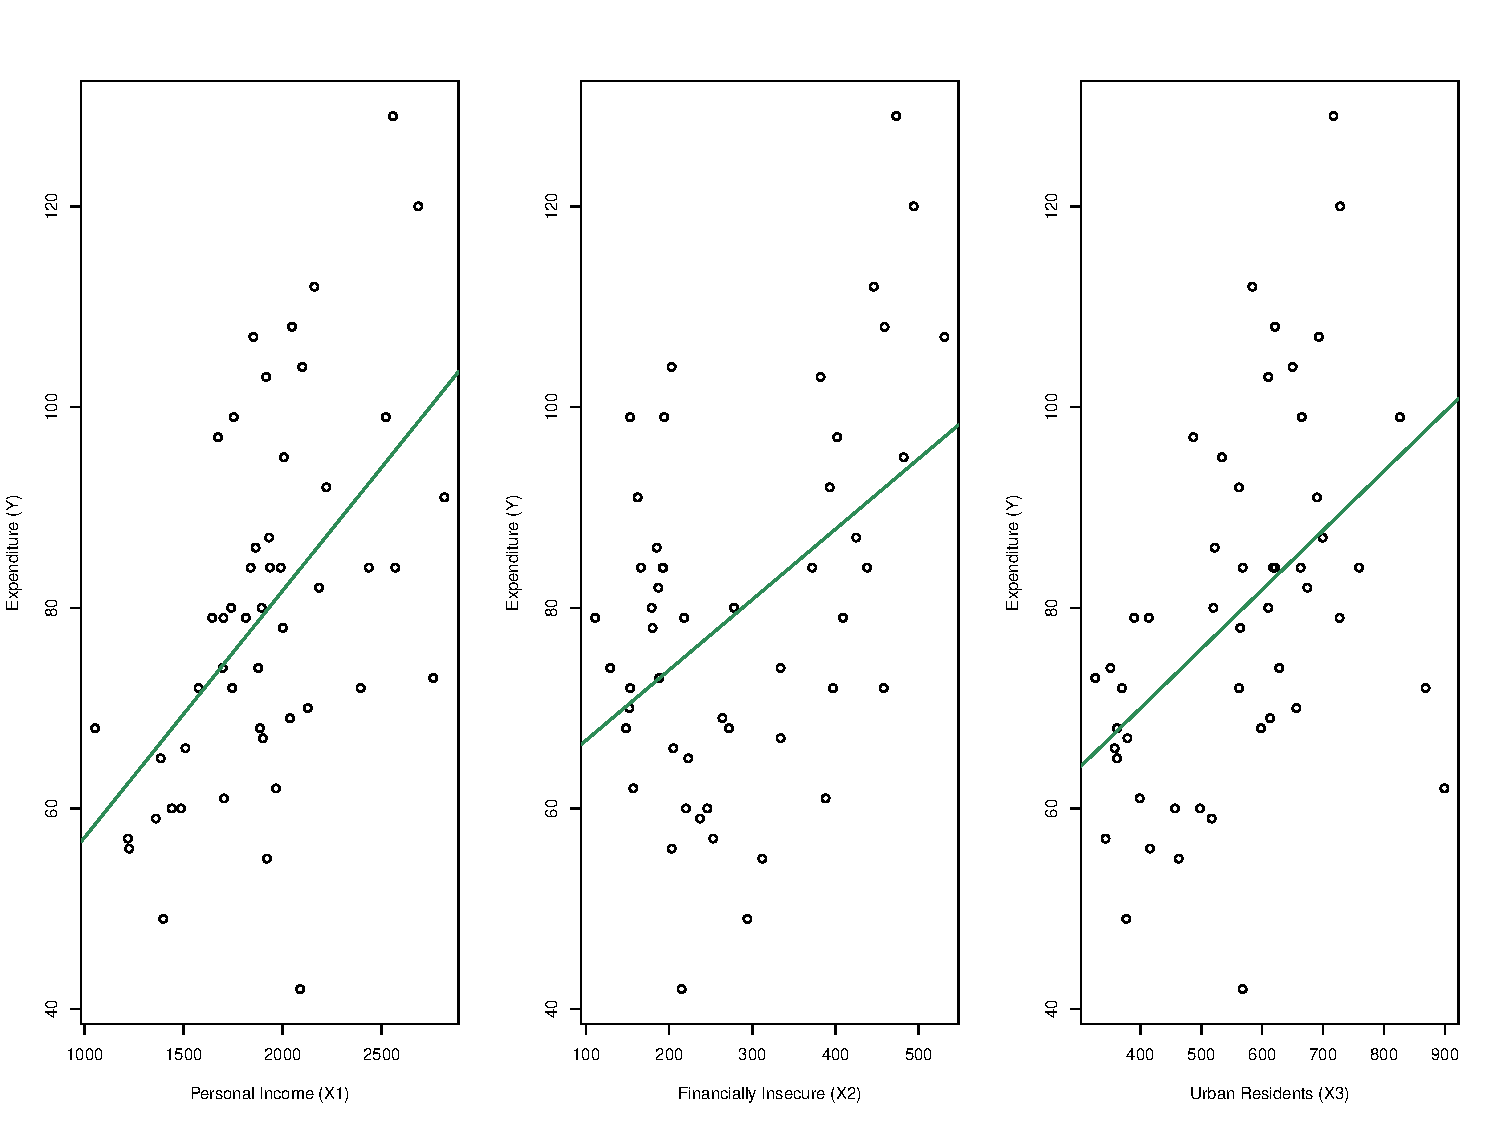
\includegraphics[width=.85\textwidth]{Relationships_1.pdf}
\end{figure}

% the code
\lstinputlisting[language=R, firstline=116, lastline=122]{PS01_answers_EGL.R}

% the plot
\begin{figure}[H]
	\centering
	\caption{\footnotesize Scatterplot of Relationships between Predictors}
	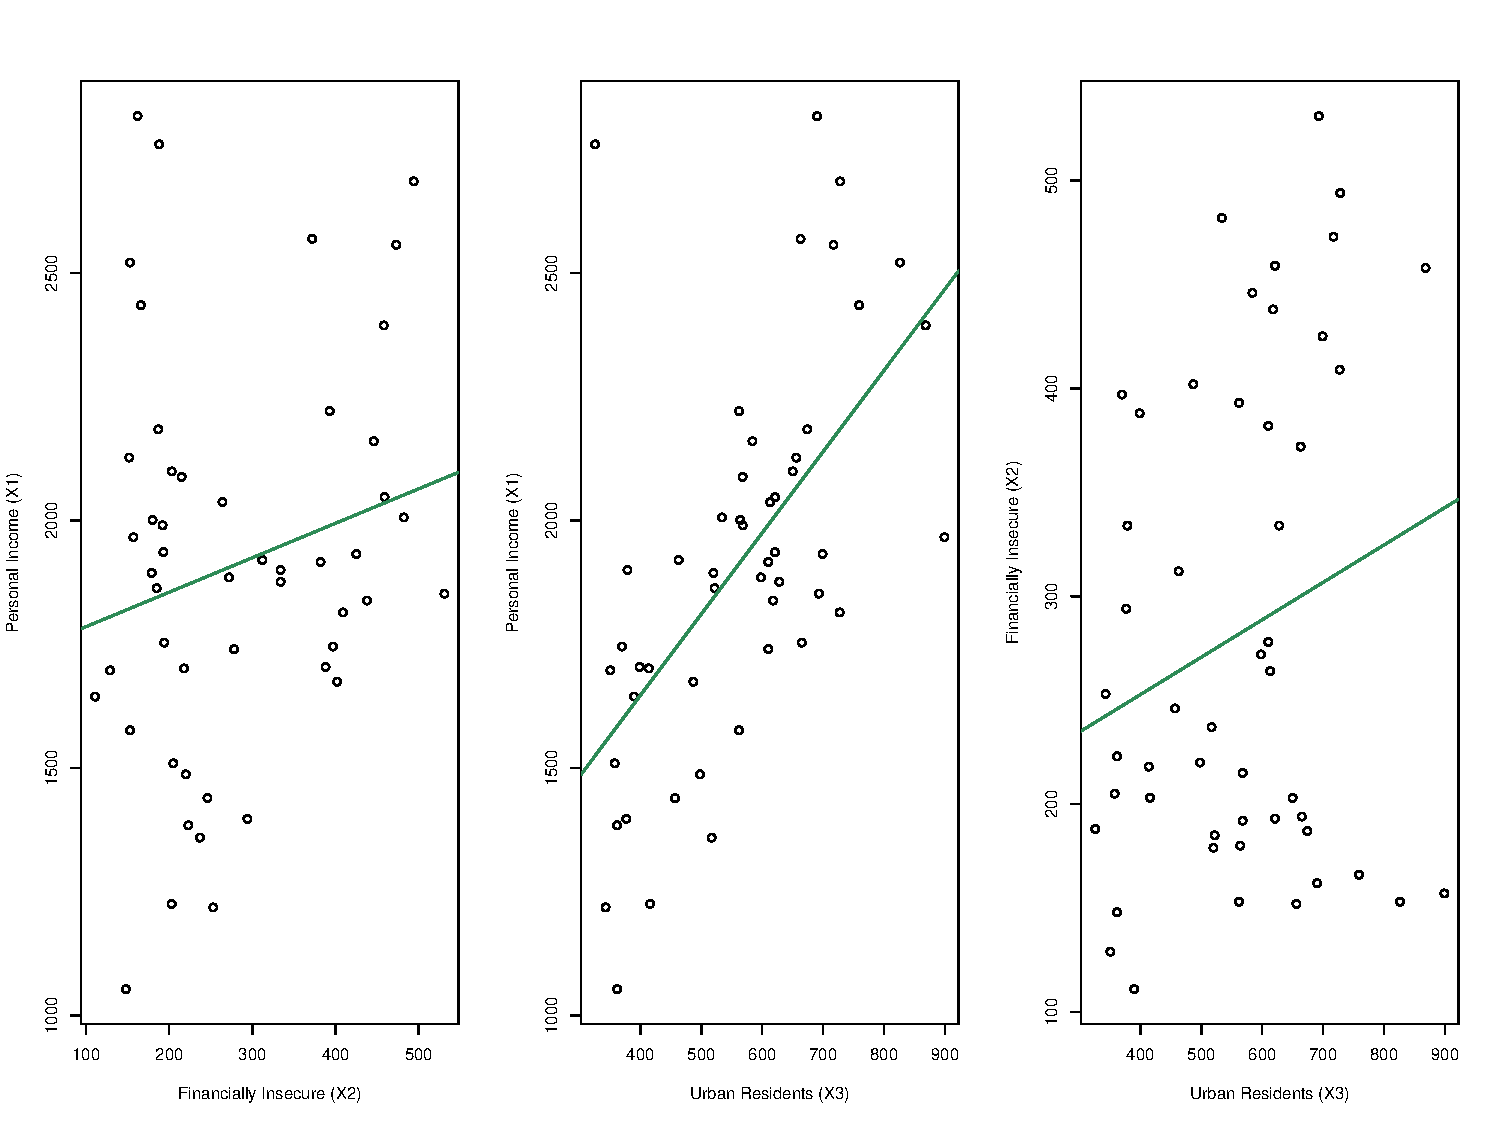
\includegraphics[width=.85\textwidth]{Relationships_2.pdf}
\end{figure}

% the code
\lstinputlisting[language=R, firstline=129, lastline=132]{PS01_answers_EGL.R}

I found this graph format and the $GGally$ package from the 'Correlogram' section of \url{r-graph-gallery.com}. I am using it here because it shows scatterplots (lower triangle), density curves (diagonal), and correlation coefficients with statistical significance (upper triangle) in one succint plot. 

% the plot
\begin{figure}[H]
	\centering
	\caption{\footnotesize Correlation Plot}
	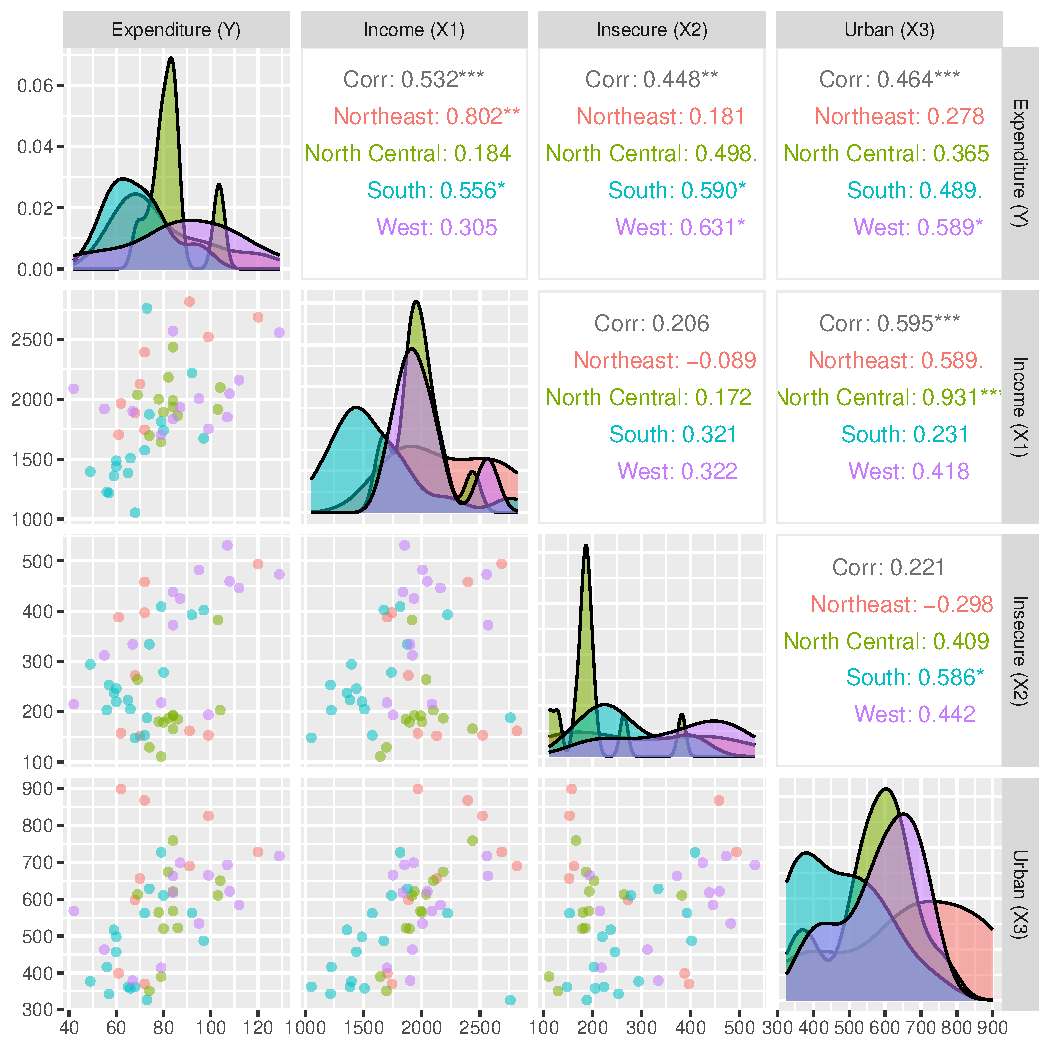
\includegraphics[width=.85\textwidth]{Correlation_Plot.pdf}
\end{figure}

Overall, all correlations are positive, which we can confirm with the cor() function:

\lstinputlisting[language=R, firstline=135, lastline=135]{PS01_answers_EGL.R}
\begin{verbatim}
	[1] 0.5317212
	[1] 0.4482876
	[1] 0.4636787
\end{verbatim}

\lstinputlisting[language=R, firstline=136, lastline=136]{PS01_answers_EGL.R}
\begin{verbatim}
	[1] 0.2056101
	[1] 0.5952504
\end{verbatim}

\lstinputlisting[language=R, firstline=137, lastline=137]{PS01_answers_EGL.R}
\begin{verbatim}
	[1] 0.2210149
\end{verbatim}

\textbf{Expenditure (Y)} is moderately and positively related to all three
predictors: income (X1) ($r = 0.53$, $p<0.001$), financial insecurity (X2)
($r = 0.45$, $p<0.01$), and urbanisation (X3) ($r = 0.46$, $p<0.001$).
States with higher income, more financially insecure residents, and larger
urban populations tend to spend more on housing assistance, which stands to reason. It's also worth noting that Y and X1 display the strongest relationship in the Northeast States ($r = 0.80$), and are weakest in North Central States ($r = 0.18$).

\textbf{Among the predictors (X1, X2, X3),} income and urbanisation are the most strongly related ($r = 0.60$, $p<0.001$). Income and insecurity ($r = 0.21$) and
urbanisation and insecurity ($r = 0.22$) are only weakly related and not
statistically significant. \\

\item %2
\textbf{Please plot the relationship between \emph{Y} and \emph{Region}? On average, which region has the highest per capita expenditure on housing assistance?}
\vspace{.5cm}

\lstinputlisting[language=R, firstline=144, lastline=152]{PS01_answers_EGL.R}

I removed the legend because it was redundant with the label for the X axis. I also added a red point for the mean of each region using stat\_summary(). 

\begin{figure}[H]
	\centering
	\caption{\footnotesize Box Plot}
	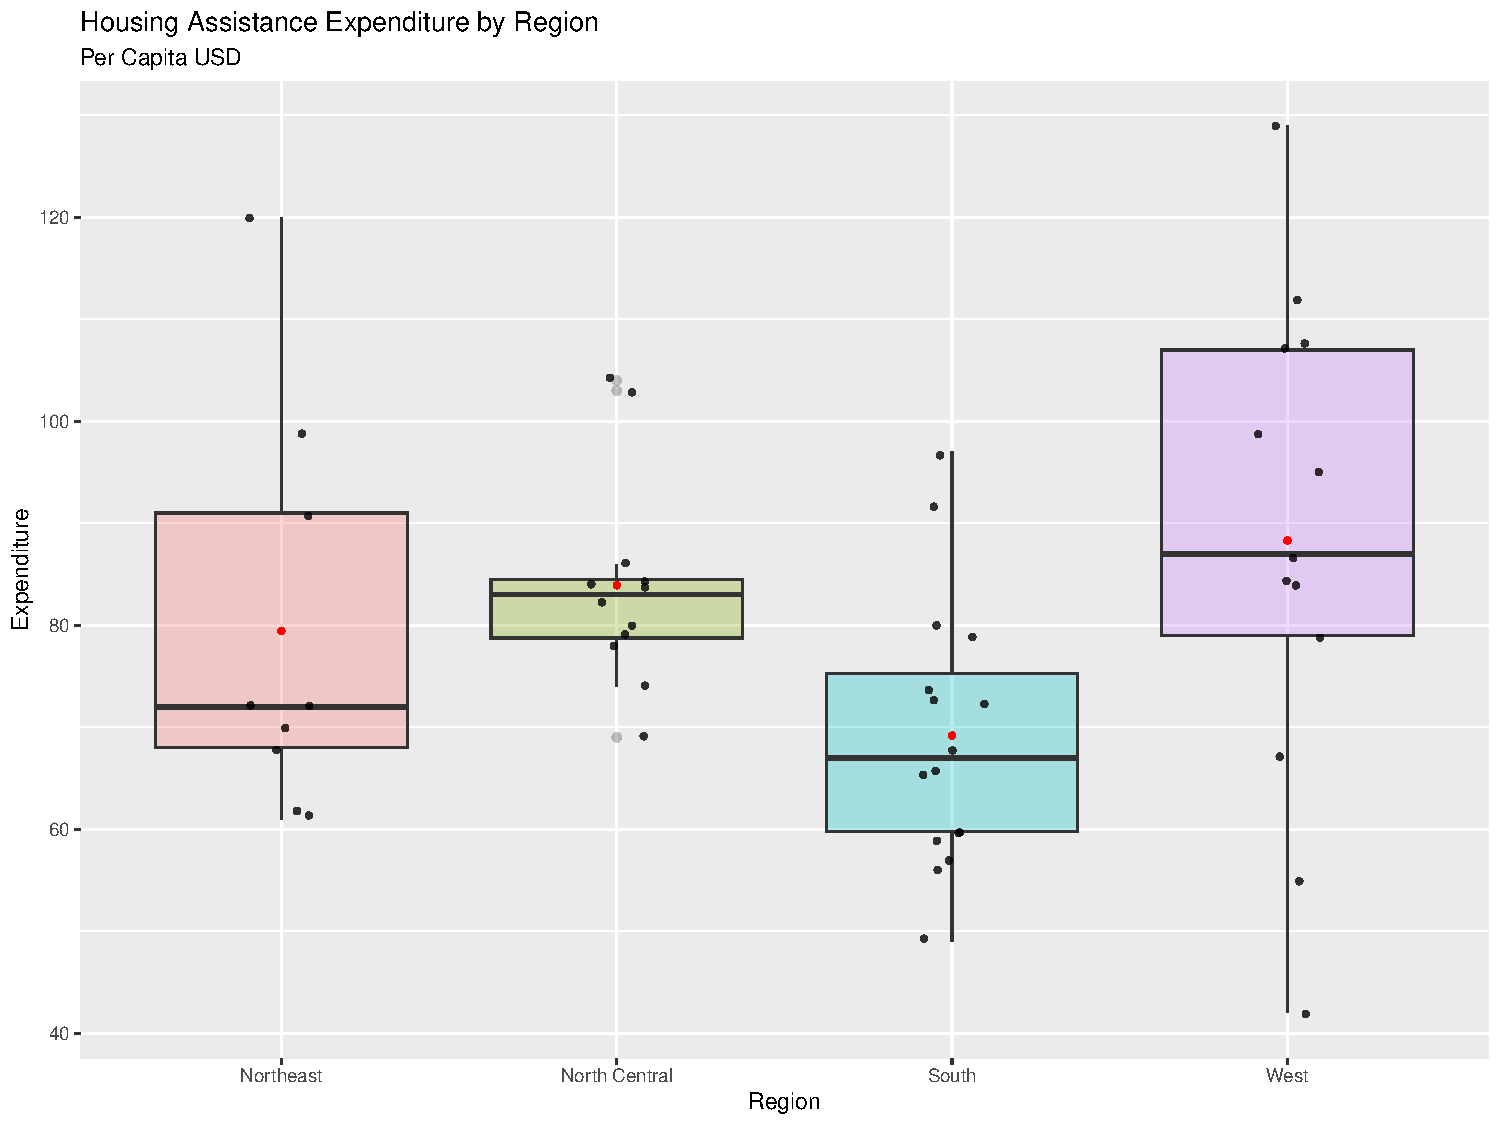
\includegraphics[width=.85\textwidth]{Box_Plot.pdf}
\end{figure}

Using the box plot, we can surmise that the Western States have the highest per capita expenditure on housing assistance with a mean of approximately 88. \\

\item %3
\textbf{Please plot the relationship between \emph{Y} and \emph{X1}? Describe this graph and the relationship. Reproduce the above graph including one more variable \emph{Region} and display different regions with different types of symbols and colors.}
 
 % the code
\lstinputlisting[language=R, firstline=160, lastline=167]{PS01_answers_EGL.R}

% the graph
\begin{figure}[H]
	\centering
	\caption{\footnotesize Scatter Plot}
	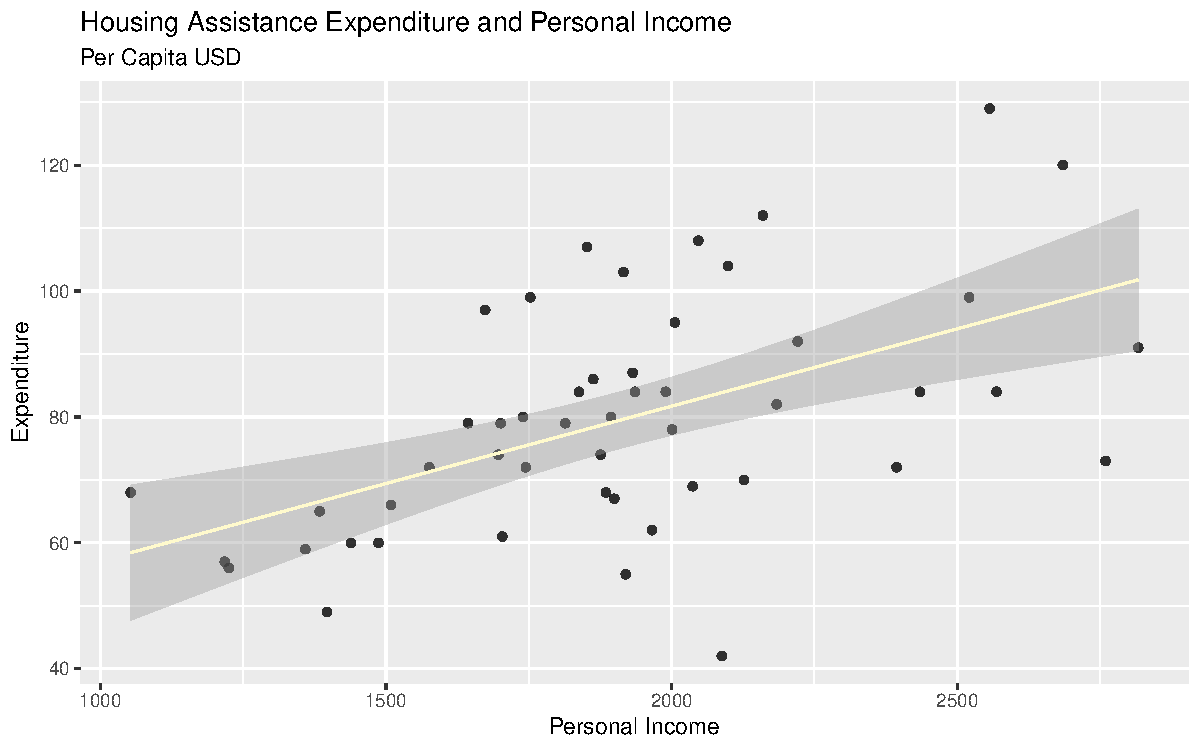
\includegraphics[width=.85\textwidth]{Scatter_Plot_1.pdf}
\end{figure}

This is a scatterplot with the line of best fit in yellow ("lemonchiffon") and the 95\% confidence interval for the regression line shaded in a grey band. It shows a positive linear relationship between personal income and expenditure.

\vspace{.5cm}

To reproduce the above graph with Region, I added symbols and colours to the geom points.\\

% the code
\lstinputlisting[language=R, firstline=177, lastline=186]{PS01_answers_EGL.R}

% the plot
\begin{figure}[H]
	\centering
	\caption{\footnotesize Scatter Plot with Regions}
	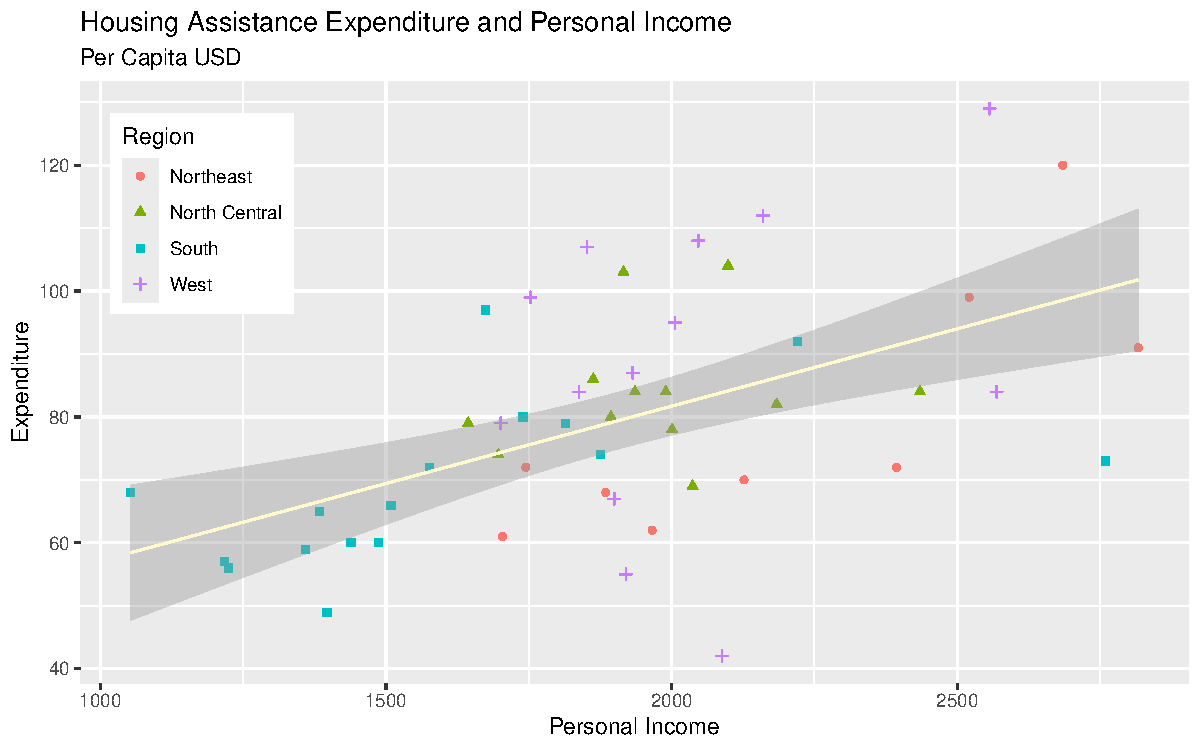
\includegraphics[width=.85\textwidth]{Scatter_Plot_2.pdf}
\end{figure}

% the analysis
With the Regions distinguished by shape and colour, we can observe that the Northeast States (red circles) have wide variance in both personal income and expenditure. It also has the fewest observations, which allow a few extreme values to skew the mean heavily. This is reflected in both the Box Plot above (Figure 4) and this scatter plot, but especially evident in the box plot where the median is considerably lower than the mean, and the difference between the two are the most pronounced of the four regions. 

The North Central States (green triangles) displays the least variance and is heavily concentrated in the middle, which was indicated by its short box and second-highest mean in Figure 4.

The Southern States (blue squares) are mostly concentrated in the bottom-left, indicating both low personal income and expenditure on shelters and housing assistance. This aligns with Figure 4, where the South had the lowest mean. 

The Western States (purple crosses) display a wide variance. This also aligns with our findings from Figure 4, where the West had the tallest box and highest mean. 

\end{itemize}


\end{document}
